\documentclass[crop,tikz]{standalone}% 'crop' is the default for v1.0, before it was 'preview'
%\usetikzlibrary{...}% tikz package already loaded by 'tikz' option
\begin{document}
\usetikzlibrary{shapes,snakes}
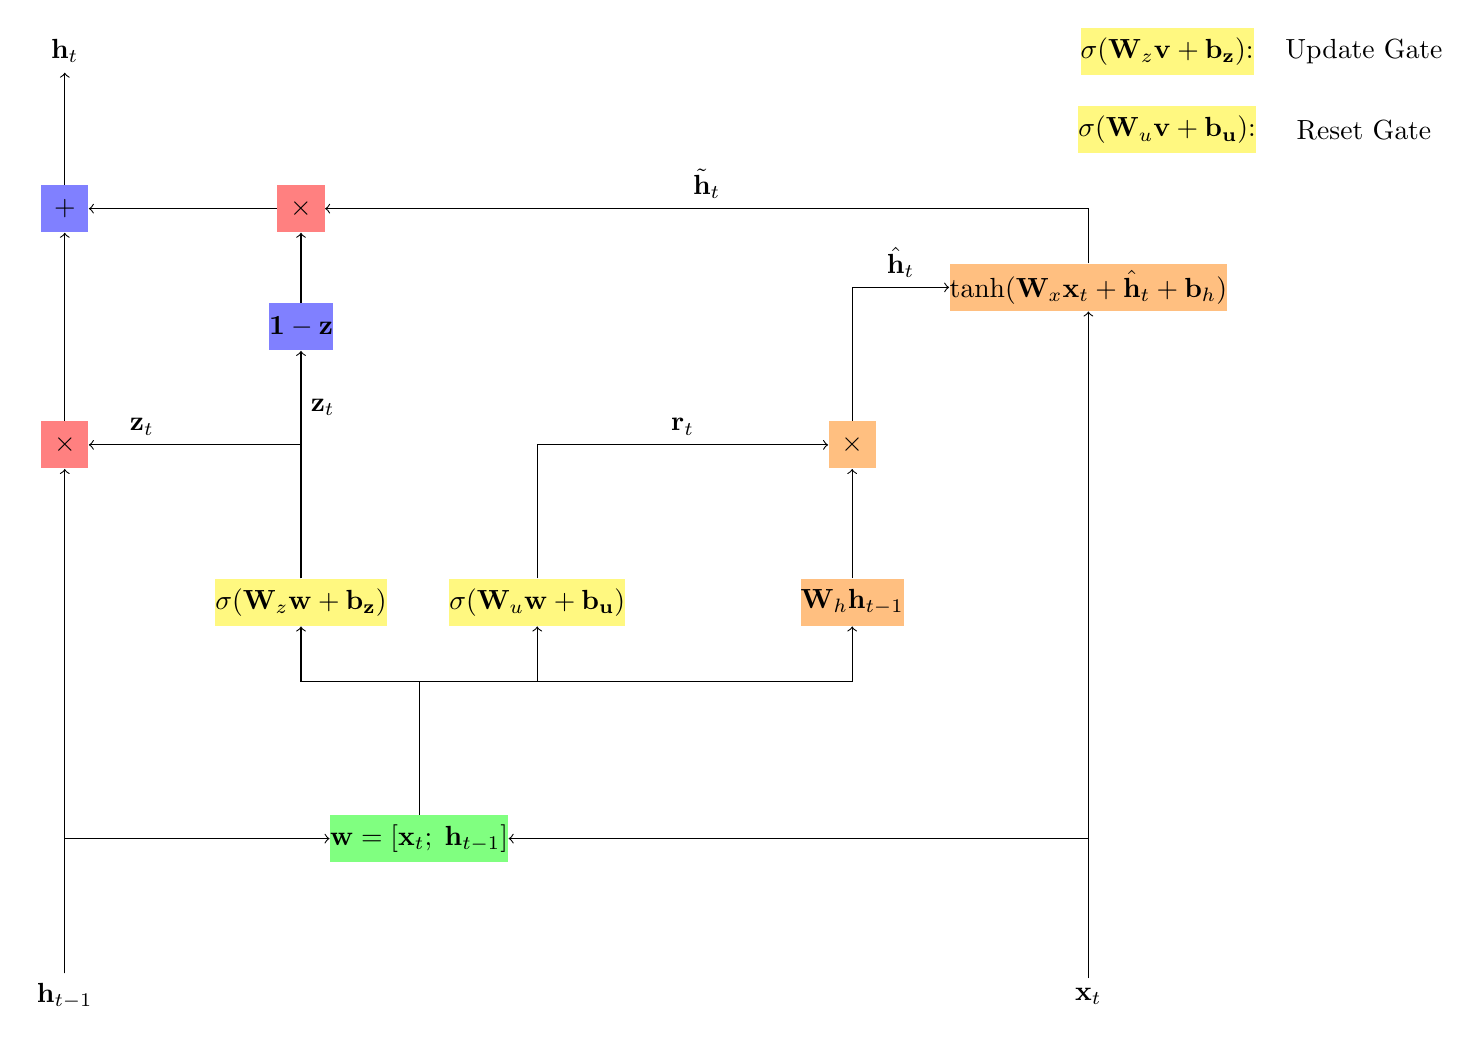
\begin{tikzpicture}
\tikzstyle{gate}=[rectangle,fill=yellow!50,minimum size=17pt,inner sep=0pt]
\tikzstyle{tanGate}=[rectangle,fill=orange!50,minimum size=17pt,inner sep=0pt]
\tikzstyle{fun}=[ellipse,fill=orange!50,minimum size=17pt,inner sep=0pt]
\tikzstyle{merge}=[rectangle,fill=green!50,minimum size=17pt,inner sep=0pt]
\tikzstyle{times}=[rectangle,fill=red!50,minimum size=17pt,inner sep=0pt]
\tikzstyle{plus}=[rectangle,fill=blue!50,minimum size=17pt,inner sep=0pt]

%get labels.
\node[gate] (fSigLabel) at (14,12) {$\sigma(\mathbf{W}_z \mathbf{v} + \mathbf{b_z})$:};\node at (16.5,12) {Update Gate};
\node[gate] (iSigLabel) at (14,11) {$\sigma(\mathbf{W}_u \mathbf{v} + \mathbf{b_u})$:};\node at (16.5,11) {Reset Gate};
%\node[gate] (oSigLabel) at (14,10) {$\sigma(\mathbf{W}_o \mathbf{z} + \mathbf{b}_o)$:};\node at (16.5,10) {Output Gate};


\node (hOld) at (0,0) {$\mathbf{h}_{t-1}$};
\node (x)    at (13,0) {$\mathbf{x}_t$};


\node[merge] (mergeW) at (4.5,2) {$\mathbf{w} = [\mathbf{x}_t; \; \mathbf{h}_{t-1}]$};
\draw[->] (x) |- (mergeW);
\draw[->] (hOld) |- (mergeW);

\node[gate] (rSig) at (3,5) {$\sigma(\mathbf{W}_z \mathbf{w} + \mathbf{b_z})$};
\node[gate] (hSig) at (6,5) {$\sigma(\mathbf{W}_u \mathbf{w} + \mathbf{b_u})$};
\node[tanGate] (preNonLin) at (10,5) {$\mathbf{W}_{h} \mathbf{h}_{t-1}$};

\node[tanGate] (rMul) at (10,7) {$\times$};

\draw[->] (mergeW) -- (4.5,4) -- (3,4) -- (rSig);
\draw[->] (mergeW) -- (4.5,4) -- (6,4) -- (hSig);
\draw[->] (mergeW) -- (4.5,4) -- (10,4) -- (preNonLin);
\draw[->] (preNonLin) -- (rMul);

\draw[->] (hSig) |- (rMul) node[near end, above] {$\mathbf{r}_t$};
\node[tanGate] (hBar) at (13,9) {$\tanh(\mathbf{W}_{x} \mathbf{x}_t + \hat{\mathbf{h}}_t + \mathbf{b}_h)$};
\draw[->] (x) -- (hBar);
\draw[->] (rMul) |- (hBar) node[near end, above] {$\hat{\mathbf{h}}_t$};


\node[plus] (invR) at (3,8.5) {$\mathbf{1} - \mathbf{z}$};

\node[times] (rtimeshOld) at (0,7) {$\times$};
\draw[->] (rSig) -- (3,7) -- (rtimeshOld) node[near end, above] {$\mathbf{z}_t$};
\draw[->] (hOld) -- (rtimeshOld);
% \draw[->] (fSig) |- (ftimesCOld) ;

\node[times] (hBarTimesrt) at (3,10) {$\times$};
\draw[->] (rSig) -- (invR) node[near end, right] {$\mathbf{z}_t$};
\draw[->] (invR) -- (hBarTimesrt);
\draw[->] (hBar) |- (hBarTimesrt) node[near end, above] {$\tilde{\mathbf{h}}_t$};


% \draw[->] (iSig) -- (ctBarTimesIt) node[near end, left] {$\mathbf{i}_t$};
% \draw[->] (ctBar) |- (ctBarTimesIt) node[near end, above] {$\bar{\mathbf{s}}_t$};

\node[plus] (compht) at (0,10) {$+$};
\draw[->] (rtimeshOld) -- (compht);
\draw[->] (hBarTimesrt) -- (compht);


\node (ht) at (0,12) {$\mathbf{h}_t$};
\draw[->] (compht) -- (ht);


% \node[merge] (mergeZ) at (11,9) {$\mathbf{z} = [\mathbf{x}_t \; \mathbf{h}_{t-1} \; \mathbf{s}_{t}]^T$};

% %draw the stateTanh and its connecting arrow
% \node[fun] (stateTanh) at (4,10) {$\tanh(\mathbf{s}_t)$};
% \draw[->] (compCt) -- (0,9) -- (4,9) -- (stateTanh);


% \node[gate] (oSig) at (11,10) {$\sigma(\mathbf{W}_o \mathbf{z} + \mathbf{b}_o)$};
% \draw[->] (mergeW) -- (11,3) -- (mergeZ);
% \draw[->] (mergeZ) -- (oSig);
% \draw[->] (compCt) -- (0,9) -- (4,9) -- (mergeZ);

% \node[times] (compHt) at (7.5,11) {$\times$};
% \draw[->] (stateTanh) |- (compHt);
% \draw[->] (oSig) |- (compHt) node[near end, above] {$\mathbf{o}_t$};

% \node (ht) at(7.5,12) {$\mathbf{h}_t$};
% \draw[->] (compHt) -- (ht);

\end{tikzpicture}
\end{document}